\PassOptionsToPackage{unicode}{hyperref}
\PassOptionsToPackage{naturalnames}{hyperref}
\documentclass[a4paper,
               bibliography=totoc,
%                draft=true,
               hidelinks,
               listof=totoc,
               twoside]{scrreprt}
\usepackage[bottom = 3 cm]{geometry}
\usepackage[
  %automark,
  %autooneside=false,% <- needed if you want to use \leftmark and \rightmark in a onesided document
  headsepline %line below header
]{scrlayer-scrpage}
%adds page numbers to center of foot on first chapter page
%\deftripstyle{ChapterStyle}{}{}{}{}{\pagemark}{}
%\renewcommand*{\chapterpagestyle}{ChapterStyle}
%deletes default footer page numbers
\clearpairofpagestyles
%customize header
\ihead{\leftmark}
\ohead{\ifstr{\leftmark}{\rightbotmark}{}{\rightbotmark}}
\lehead{\pagemark}
%right-handed even page headers
\rehead{\headmark}
\lohead{\headmark}
\rohead{\pagemark}
%add section title to header
\automark[section]{chapter}

\usepackage[main=english, ngerman]{babel}
\usepackage[utf8]{inputenc}
\usepackage[T1]{fontenc}
\usepackage{microtype}
\usepackage[onehalfspacing]{setspace}
\usepackage{pdfpages}
\usepackage{lipsum}
\usepackage{etoolbox}
\usepackage{chemformula}
\usepackage{simpler-wick}
\usepackage{listings}
\usepackage{bbold}
\usepackage{physics}
\usepackage{amsmath}
\usepackage{bm}
\usepackage{xspace}

\clubpenalty10000
\widowpenalty10000

\usepackage[perpage, symbol*]{footmisc}

% uncomment if you want to start next chapter on same page
% \usepackage{etoolbox}
% \makeatletter
% \patchcmd{\scr@startchapter}{\if@openright\cleardoublepage\else\clearpage\fi}{}{}{}
% \makeatother

%for enumeration environment used for own publication list
\usepackage[inline]{enumitem}
  \setlist[itemize]{itemsep=10pt, label={--}}

\usepackage{graphicx}
\usepackage[labelfont=bf, labelsep=space, format=plain]{caption}

%for tabular for appended publications
\usepackage{array}
  \newcolumntype{T}{>{\ttfamily}l}
%   \newcolumntype{L}[1]{>{\raggedright\let\newline\\\arraybackslash\hspace{0pt}  }m{#1}}
  \newcolumntype{L}[1]{>{\raggedright\setlength{\parindent}{-0.3cm}\let\newline\\\arraybackslash\hspace{0pt}}m{#1}}


\usepackage{hyperref} %has to be loaded before glossaries package for hyperlinks of acronyms to work!
\usepackage[acronym, toc, nopostdot]{glossaries}
\usepackage{glossary-longbooktabs}
  \newcommand*\myglsfirst[1]{\glsfirst{#1}\glsunset{#1}}
  \newcommand*\myglsfirstplural[1]{\glsfirstplural{#1}\glsunset{#1}}
  \renewcommand*\glspostdescription{\hfill}
\usepackage{glossaries-prefix}
\newacronym{cc-pV$X$Z}{cc-pV$X$Z}{correlation-consistent polarised valence with $X$-zeta quality ($X$=D, T, Q, 5, 6, ...)}
\newacronym{aug-cc-pV$X$Z}{cc-pV$X$Z}{correlation-consistent polarised valence with $X$-zeta quality ($X$=D, T, Q, 5, 6, ...) augmented with diffuse functions}
\newacronym{cc-pCV$X$Z}{cc-pV$X$Z}{correlation-consistent polarised valence with $X$-zeta quality ($X$=D, T, Q, 5, 6, ...) with core correlation}
\newacronym{ECG}{ECG}{Explicitly Correlated Gaussian}
\newacronym{GTG}{GTG}{Gaussian-type Geminal}
\newacronym{MC}{MC}{Monte Carlo}
\newacronym{API}{API}{application programming interface}
\newacronym{SI}{SI}{supporting information}
\newacronym{DTN}{DTN}{Drummond-Towler-Needs}
\newacronym{MAE}{MAE}{mean absolute error}
\newacronym{MAD}{MAD}{mean absolute deviation}
\newacronym{RMSD}{RMSD}{root mean squared deviation}
\newacronym{MD}{MD}{mean deviation}
\newacronym{MaxD}{MaxD}{maximum deviation}
\newacronym{DF}{DF}{density fitting}
\newacronym{RI}{RI}{resolution of identity}
\newacronym{DIIS}{DIIS}{direct inversion of the iterative subspace}
\newacronym{ITF}{ITF}{integrated tensor framework}
\newacronym{CTF}{CTF}{cyclops tensor framework}
\newacronym{CT}{CT}{charge transfer}
\newacronym{QC}{QC}{quantum chemistry}
\newacronym{BOA}{BOA}{Born-Oppenheimer approximation}
\newacronym{SE}{SE}{Schrödinger equation}
\newacronym{STO}{STO}{Slater-type orbitals}
\newacronym{GTO}{GTO}{Gaussian-type orbitals}
\newacronym{AO}{AO}{atomic orbital}
\newacronym{MO}{MO}{molecular orbital}
\newacronym{LCAO}{LCAO}{linear combination of atomic orbitals}
\newacronym{SALC}{SALC}{symmetry adapted linear combination}
% \newacronym{vdz}{\textsc{vdz}}{cc-pVDZ}
% \newacronym{avdz}{\textsc{avdz}}{aug-cc-pVDZ}
% \newacronym{vtz}{\textsc{vtz}}{cc-pVTZ}
% \newacronym{avtz}{\textsc{avtz}}{aug-cc-pVTZ}
\newacronym{CBS}{CBS}{complete basis set}
\newacronym{OBS}{OBS}{orbital basis set}
\newacronym{ABS}{ABS}{auxiliary basis set}
\newacronym{CABS}{CABS}{complementary auxiliary basis set}
\newacronym{BSSE}{BSSE}{basis set superposition error}
\newacronym{BSIE}{BSIE}{basis set incompleteness error}
\newacronym{CSF}{CSF}{configuration state function}
\newacronym{SD}{SD}{Slater determinant}
\newacronym{OSS}{OSS}{open-shell singlet}
\newacronym{SCF}{SCF}{self consistent field}
\newacronym{HF}{HF}{Hartree-Fock}
\newacronym{RHF}{RHF}{restricted Hartree-Fock}
\newacronym{ROHF}{ROHF}{restricted open-shell Hartree-Fock}
\newacronym{UHF}{UHF}{unrestricted Hartree-Fock}
\newacronym{QRHF}{QRHF}{quasi restricted Hartree-Fock}
\newacronym{KS}{KS}{Kohn-Sham}
\newacronym{DFT}{DFT}{density functional theory}
\newacronym{TD}{TD}{time dependant}
\newacronym{CAS}{CAS}{complete active space}
\newacronym{IAS}{IAS}{incomplete active space}
\newacronym{MCSCF}{MCSCF}{multiconfigurational self-consistent field}
\newacronym{CASSCF}{CASSCF}{complete active space self-consistent field}
\newacronym{QMC}{QMC}{quantum Monte Carlo}
\newacronym{VMC}{VMC}{variational Monte Carlo}
\newacronym{DMC}{DMC}{diffusion Monte Carlo}
\newacronym{PT}{PT}{perturbation theory}
\newacronym{MP2}{MP2}{second-order M{\o}ller-Plesset perturbation theory}
\newacronym{BCH}{BCH}{Baker-Campbell-Hausdorff}
\newacronym{SR}{SR}{single reference}
\newacronym{MR}{MR}{multireference}
\newacronym{HS}{HS}{Hilbert space}
\newacronym{FS}{FS}{Fock space}
\newacronym{SU}{SU}{state universal}
\newacronym{SS}{SS}{state specific}
\newacronym{DSRG}{DSRG}{driven similarity renormalization group}
\newacronym{ic}{ic}{internally contracted}
\newacronym{CC}{CC}{coupled cluster}
\newacronym{CCD}{CCD}{coupled cluster with double excitations}
\newacronym{CCSD}{CCSD}{coupled cluster with single and double excitations}
\newacronym{CCSD(T)}{CCSD(T)}{coupled cluster with single and double excitations and perturbative triples}
\newacronym{CCSDT}{CCSDT}{coupled cluster with single, double and triple excitations}
\newacronym{CCSDTQ}{CCSDTQ}{coupled cluster up to quadruple excitations}
\newacronym{DC}{DC}{distinguishable cluster}
\newacronym{DCD}{DCD}{distinguishable cluster with double excitations}
\newacronym{DCSD}{DCSD}{distinguishable cluster with single and double excitations}
\newacronym{2D}{2D}{two determinant}
\newacronym{DC-CCSDT}{DC-CCSDT}{distinguishable cluster with single, double and triple excitations}
\newacronym{EOM}{EOM}{equation of motion}
\newacronym{SF}{SF}{spin flip}
\newacronym{LR}{LR}{linear response}
\newacronym{FR}{FR}{fixed reference}
\newacronym{CI}{CI}{configuration interaction}
\newacronym{sCI}{sCI}{selected configuration interaction}
\newacronym{exFCI}{exFCI}{extrapolated selected configuration interaction of \gls{FCI} quality}
\newacronym{exSHCI}{exSHCI}{extrapolated semi-stochastic heat bath configuration interaction}
\newacronym[first={MRCI}]{MRCI}{MRCI}{multi reference configuration interaction}
\newacronym{ED}{ED}{exact diagonalization}
\newacronym{FCI}{FCI}{full configuration interaction}
\newacronym{FCIQMC}{FCIQMC}{full configuration interaction quantum Monte Carlo}
\newacronym{DMRG}{DMRG}{density matrix renormalization group}
\newacronym{TC}{TC}{transcorrelation}
\newacronym{xTC}{xTC}{transcorrelation via exclusion of explicit three-body components}
\newacronym{FROGG}{FROGG}{frozen Gaussian geminal}
\newacronym{TMM}{TMM}{trimethylenemethane}
% \newacronym{RDM}{RDM}{reduced density matrix}
\newacronym{1RDM}{1RDM}{1-electron reduced density matrix}
\newacronym{2RDM}{2RDM}{2-electron reduced density matrix}

\makeglossaries

%print Contents also in TOC
\BeforeTOCHead[toc]{\cleardoublepage\pdfbookmark{\contentsname}{toc}}
\KOMAoptions{parskip=false}% no parskip in ToC
\RedeclareSectionCommand[afterskip=1sp minus 1sp]{chapter}% no skip after ToC title
\DeclareTOCStyleEntry[beforeskip=.3cm]{chapter}{chapter}

%make binding margin on first page on left side and not on right
\let\tmp\oddsidemargin
\let\oddsidemargin\evensidemargin
\let\evensidemargin\tmp
\reversemarginpar

\usepackage[
  backend=biber,
  doi=false,
  giveninits=false,
  isbn=false,
  url=false,
  articletitle=true,
  chaptertitle=true,
  style=chem-acs,
  maxbibnames=99,
  maxcitenames=99,
  urldate=iso,
  seconds=true
]{biblatex}

%make title in bib hyperlink to doi
\newbibmacro{string+doi}[1]{%
  \iffieldundef{doi}{#1}{\href{https://doi.org/\thefield{doi}}{#1}}}
\DeclareFieldFormat{title}{\usebibmacro{string+doi}{\mkbibemph{#1}}}
\DeclareFieldFormat[article]{title}{\usebibmacro{string+doi}{\mkbibquote{#1}}}

\usepackage{csquotes}
\DeclareFieldFormat{title}{\textit{#1}}
\DeclareFieldFormat{booktitle}{\textit{#1}}
\DeclareFieldFormat{journaltitle}{\upshape{#1}}
\DeclareFieldFormat{citetitle}{#1}

% add bib files like so -- make sure to keep categorised!
% \addbibresource{./library/[...].bib}
% \addbibresource{library/mypapers.bib}
% \addbibresource{library/*.bib}


\addbibresource{library/Textbooks.bib}
\addbibresource{library/Benchmarks.bib}
\addbibresource{library/F12.bib}
\addbibresource{library/FCIQMC.bib}
\addbibresource{library/H chain.bib}
\addbibresource{library/Misc.bib}
\addbibresource{library/mypapers.bib}
\addbibresource{library/N2.bib}
\addbibresource{library/Sign Problem.bib}
\addbibresource{library/Software.bib}
\addbibresource{library/TC-General-Resurgence.bib}
\addbibresource{library/Textbooks.bib}
\addbibresource{library/Basis set_Extrapolation.bib}
\addbibresource{library/Standard Methods.bib}
\addbibresource{library/cusp conditions.bib}
\addbibresource{library/TC.bib}
\addbibresource{library/MC.bib}

\let\cite\supercite

%for onlinecite
\DeclareCiteCommand{\citenum}
  {}
  {\bibhyperref{\printfield{labelnumber}}}
  {}
  {}

\makeatletter
  \newrobustcmd*{\setmaxcitenames}{\numdef\blx@maxcitenames}
\makeatother

%define thesis title etc.

% meta-data variables
\newcommand*{\thetitle}{%
  Development of the Transcorrelated Full Configuration Interaction Quantum Monte Carlo Method
}

\newcommand*{\theapproval}{%
  Von der Fakultät Chemie der Universität Stuttgart zur Erlangung der Würde eines
    Doktors der Naturwissenschaften (Dr.\@ rer.\@ nat.\@) genehmigte Abhandlung
}
\newcommand*{\theauthor}{Jacobus Philip Haupt}
\newcommand*{\thebirthplace}{George, S\"udafrika}
\newcommand*{\thedefensedate}{....................}
\newcommand*{\thedate}{19 September 2024}
\newcommand*{\theyear}{2024}
\newcommand*{\theuniversity}{Universität Stuttgart}
\newcommand*{\theinstitute}{Max-Planck-Institut für Festkörperforschung, Stuttgart}
\newcommand*{\theadvisor}{Prof.\@ Dr.\@ Ali Alavi}
\newcommand*{\theexamineri}{Prof.\@ Dr.\@ Andreas Köhn}
\newcommand*{\theexaminerii}{Prof.\@ Dr.\@ Joris van Slageren}

%define custom commands
\newcommand{\onlinecite}[1]{Ref.~\citenum{#1}}
\newcommand{\onlinecites}[2]{Refs.~\citenum{#1}, \citenum{#2}}
\newcommand{\onlinecitess}[3]{Refs.~\citenum{#1}, \citenum{#2}, \citenum{#3}}
\newcommand{\todo}[1]{{\color{red}TODO: #1}}
\newcommand*\ownref[1]{Ref.~\textbf{\ref{#1}}}
\newcommand*\superownref[1]{\textsuperscript{\textbf{\ref{#1}}}}
\newcommand{\eq}[1]{Eq.~(\ref{#1})}
\newcommand{\eqs}[2]{Eqs.~(\ref{#1},~\ref{#2})}
\newcommand{\chap}[1]{chapter~\ref{#1}}
\newcommand{\sect}[1]{sec.~\ref{#1}}
\newcommand{\fig}[1]{Figure~\ref{#1}}
\newcommand{\tab}[1]{Table~\ref{#1}}
\newcommand{\NL}{\nonumber \\}
\newcommand{\nl}{\nonumber \\ & }
\newcommand{\avxz}[1]{aug-cc-pV{#1}Z\xspace}
\newcommand{\vxz}[1]{cc-pV{#1}Z\xspace}
\newcommand{\avdz}{\avxz{D}}
\newcommand{\vdz}{\vxz{D}}
\newcommand{\avtz}{\avxz{T}}
\newcommand{\vtz}{\vxz{T}}
\newcommand{\avqz}{\avxz{Q}}
\newcommand{\vqz}{\vxz{Q}}
% \newcommand{\av5z}{\avxz{5}}
% \newcommand{\v5z}{\vxz{5}}

\newcommand{\mathdef}{\mathrel{\mathop:}=}
\newcommand{\e}{\mathrm{e}}
\renewcommand{\d}{\mathrm{d}}
\newcommand{\htc}{\hat H_\mathrm{TC}}

\newcommand{\red}[1]{{\color{red} #1}}
\newcommand{\blue}[1]{{\color{blue} #1}}
\newcommand{\magenta}[1]{{\color{magenta} #1}}
\newcommand{\brown}[1]{{\color{brown} #1}}
\definecolor{pinegreen}{rgb}{0.0, 0.47, 0.44}
\newcommand{\green}[1]{{\color{pinegreen} #1}}

\newcommand{\neci}{\texttt{NECI}\xspace}
\newcommand{\molpro}{\texttt{Molpro}\xspace}
\newcommand{\casino}{\texttt{CASINO}\xspace}
\newcommand{\pyscf}{\texttt{pyscf}\xspace}
\newcommand{\tchint}{\texttt{tchint}\xspace}
\newcommand{\pytchint}{\texttt{pytchint}\xspace}
% \newcommand{\github}{GitHub }
\newcommand{\quantumpackage}{\texttt{quantum package}\xspace}
\newcommand{\dice}{\texttt{dice}\xspace}
\newcommand{\quest}{\texttt{quest}\xspace}
\newcommand{\elemcojl}{\texttt{ElemCo.jl}\xspace}
\newcommand{\quantwo}{\texttt{Quantwo}\xspace}
\newcommand{\ccdiag}{\texttt{ccdiag}\xspace}
\newcommand{\wicked}{\texttt{Wick}\&\texttt{d}\xspace}
\newcommand{\pdgq}{\texttt{p$^\dg$q}}

\newcommand{\hartree}{$E_\mathrm{h}$}
\newcommand{\Ms}{M_\mathrm{s}}
\newcommand{\ac}[1]{\ensuremath{a_{#1}^\dagger}}
\newcommand{\ad}[1]{\ensuremath{a_{#1}}}
\newcommand{\el}{}

\newcommand{\mat}{\mathbf}
% \newcommand{\op}[1]{\hat{\mathrm{#1}}}
\newcommand{\dg}{\dagger}
\newcommand{\half}{\frac{1}{2}}
\newcommand{\third}{\frac{1}{3}}
\newcommand{\quart}{\frac{1}{4}}
% \DeclareMathOperator\erf{erf}
% Define \lt and \gt for `less than' and `greater than'
\mathchardef\lt="313C \mathchardef\gt="313E
% Set up `<' and `>' as angle brackets
% \mathcode`<="4268 \mathcode`>="5269
% \newcommand{\bra}{{\texttt bra }}
% \newcommand{\ket}{{\texttt ket }}
%\newcommand{\Perm}[2]{{\cal P}\left(#1,#2\right)}
\newcommand{\Perm}[2]{\hat{\cal P}^{#1}_{#2}}
\newcommand{\sop}[1]{{\cal S}\left(#1\right)}
\newcommand{\Sop}[2]{{\cal S}\left(#1,#2\right)}
\newcommand{\asop}[1]{{\cal A}\left(#1\right)}
\newcommand{\ASop}[2]{{\cal A}\left(#1;#2\right)}
\newcommand{\spa}[1]{{#1}}
\newcommand{\spb}[1]{\bar{#1}}

\newcommand{\one}{\mathbb{1}}

% for presubscripts and presuperscripts (e.g., \pre{^x}U_a)
\newcommand{\pre}[1]{\,#1\!}

\DeclareUnicodeCharacter{3B1}{\ensuremath{\alpha}}
\DeclareUnicodeCharacter{3B2}{\ensuremath{\beta}}
\DeclareUnicodeCharacter{3B3}{\ensuremath{\gamma}}
\DeclareUnicodeCharacter{3B4}{\ensuremath{\delta}}



%https://tex.stackexchange.com/questions/246411/koma-script-how-to-style-the-title-of-a-chapter
\KOMAoption{chapterprefix}{true}
\renewcommand*\raggedchapter{\centering}
\newif\ifmakeupper
\newcommand*\chaptertitleformat[1]{\ifmakeupper\MakeUppercase{#1}\else#1\fi}
\addtokomafont{chapter}{\makeuppertrue}
\setkomafont{chapterprefix}{\normalsize\mdseries}
\renewcommand*{\chapterformat}{%
    \MakeUppercase{\chapappifchapterprefix{\nobreakspace}}\thechapter\autodot%
    \IfUsePrefixLine{%
      \par\nobreak\vspace{-\parskip}\vspace{-.6\baselineskip}%
      \rule{0.9\textwidth}{.5pt}%
    }{\enskip}%
}
\RedeclareSectionCommand[beforeskip=0pt,afterskip=4\baselineskip]{chapter}

\renewcaptionname{english}{\contentsname}{\chaptertitleformat{Contents}}

\begin{document}

\pagenumbering{roman}
\begin{titlepage}
  \begin{spacing}{1}
    \begin{center}
      \begin{otherlanguage}{ngerman}
        % no indentation of paragraphs
        \setlength{\parindent}{0pt}

        ~\vspace{1em}

        {\bfseries\huge\thetitle\par}

        \vfill

        \theapproval

        \vfill

        Vorgelegt von

        {\bfseries\Large\theauthor\par}

        aus \thebirthplace

        \vfill

        \begin{tabular}{ll}
          Hauptberichter:   &\theadvisor\\
          Mitberichter:     &\theexamineri\\
          Prüfungsvorsitzender: &\theexaminerii\\
          \multicolumn{2}{l}{%
            Tag der mündlichen Prüfung:\quad%
            \thedefensedate%
          }
        \end{tabular}

        \vfill

        \includegraphics[width=60mm]{./figures/logos/CI_MPI_FKF_MPG_gruen.pdf}
        \hspace{1em}
        \includegraphics[width=60mm]{./figures/logos/logoUniversity}

        \vspace{2em}

        \theuniversity{}

        \vspace{1em}

        \theinstitute{}

        \vspace{1em}

        \theyear
      \end{otherlanguage}
    \end{center}
  \end{spacing}
\end{titlepage}
\cleardoublepage


% don't display page number
\thispagestyle{empty}

\vspace*{\fill}

\begin{minipage}{0.865\textwidth}%
  \begin{center}
    \begin{minipage}{0.80\textwidth}%
      \begin{flushleft}
        \textit{%
          It is important to realize that in physics today, we have no knowledge of what energy \emph{is}.
        }
      \end{flushleft}
      \begin{flushleft}
        \small--- Richard Feynman, \textit{Feynman Lectures on Physics, Volume 1, Chapter 4}
      \end{flushleft}
    \end{minipage}%
  \end{center}
\end{minipage}

\vspace*{\fill}

\cleardoublepage

% \setcounter{tocdepth}{1}
\tableofcontents
\cleardoublepage


\begin{otherlanguage}{ngerman}
\addchap{Erklärung über die Eigenständigkeit der Dissertation}

Ich erkläre hiermit an Eides statt, dass ich die vorliegende Arbeit
  \begin{quote}
    \glqq{}\textit{\thetitle{}}\grqq{}
  \end{quote}
  ohne Hilfe Dritter und ohne Benutzung anderer als der angegebenen
    Hilfsmittel angefertigt habe; die aus fremden Quellen direkt oder
    indirekt übernommenen Gedanken sind als solche kenntlich gemacht.
  Die Arbeit wurde bisher in gleicher oder ähnlicher Form in keiner anderen
    Prüfungsbehörde vorgelegt.
\end{otherlanguage}


\vspace{4cm}

\noindent\rule{5cm}{.4pt}\hfill\rule{5cm}{.4pt}\par
\noindent Datum, Ort \hfill Unterschrift

\addchap{Acknowledgements}
\todo{more detail...}

Foremost, I would like to thank my supervisor \textbf{Ali Alavi} for his guidance and undying optimism, as well as for being an excellent professional role model. Similarly, I would like to thank \textbf{Daniel Kats} for his professional guidance and patience with me as I learned the basics of electronic structure, especially at the start of my PhD while I was still working remotely from Vancouver.

I also thank \textbf{Evelin Christlmaier} for all her support, both professionally and personally, and for being a joy to work with.

My time at MPI has, to my pleasure, involved a lot of software development, and for that I am especially grateful to have had such knowledgeable coworkers as \textbf{Robert Anderson} and \textbf{Oskar Weser} to go to for advice and with whom to argue which text editor is best.

I would also like to thank my former and present coworkers \textbf{Pablo L\'opez-R\'ios}, \textbf{Aron Cohen} and \textbf{Kai Guther} for their work on making \tchint a reality. \textbf{Andreea Filip} and \textbf{Ke Liao} have been especially pivotal in making the \pytchint package possible.

While our time together in the group was short, \textbf{Werner Dobrautz} distilled in me a greater sense of mindfulness and reassurance that everything will be okay.

\todo{Also thank my committee}

\todo{Friends back home: Karan(!), Michael, Charlie, Zack, Cam, Mr Barber}

\todo{People who got me here: Roman Krems, Christian Ast(!)}

\todo{Johannes}

Finally, I want to thank my dear friends who made my time in Stuttgart infinitely more colourful: \textbf{Aybike Reyhanl\i}, \textbf{Thomas Schraivogel}, \textbf{Ingemar Schmidt}, \textbf{Rut Martinez}, \textbf{Nikos Papanikolaou}, \textbf{Martin Baumann}, and especially \textbf{Theresa Huber} with whom I shall always cherish countless hours dancing.

\printglossary[type=\acronymtype]
% \printglossary[type=\acronymtype, nonumberlist]
%\printglossary[title={Symbols}, style=long-booktabs, nonumberlist]

\cleardoublepage
\begin{otherlanguage}{ngerman}
\addchap{Zusammenfassung}

Die Transkorrelierten (TC) Methode ist eine Methode in der Quantenchemie, die in den letzten Jahren an Bedeutung gewonnen hat. In diese Methode wird eine Ähnlichkeitstransformation auf den elektronischen Hamiltonoperator angewendet, um Korrelationseffekte, insbesondere der dynamischen Korrelation, durch explizite Behandlung analytisch bekannter Eigenschaften des Hamiltonoperator zu erfassen. Diese Methode wurde bereits mit der ,,Full Configuration Interaction Quantum Monte Carlo'' (FCIQMC) Methode kombiniert, einer effizienten stochastischen Methode zur Lösung der Schrödingergleichung und zur Berechnung physikalischer Observablen. Diese Dissertation widmet sich einer vertieften Untersuchung dieser Methoden, insbesondere der TC-Methode.

Nach einer Wiederholung der Grundlagen der Quantenchemie, wird die Verwendung flexibler Jastrow-Faktoren, die in der Literatur des Variational Quantum Monte Carlos (VMC) bekannt sind, vorgestellt. Damit minimieren wir die Varianz der TC-Referenzenergie.Es zeigt sich, dass dies zu einer schnellen Basissatzkonvergenz führt und eine Genauigkeit erreicht, für die herkömmliches FCIQMC viel größere Basissätze erfordern würde. Außerdem kompaktiert dieses Minimierungsverfahren auch die Wellenfunktion, was eine effizientere FCIQMC-Berechnung ermöglicht. Im weiteren Verlauf erweitern wir die Methode für Probleme mit starken Multireferenzproblemen, insbesondere indem wir die Dissoziation des N$_2$ als Stresstest verwenden. Wir zeigen die Notwendigkeit eines Multireferenz-Jastrow-Faktor-Ansatzes auf und minimieren deshalb die Varianz eines Multireferenzzustands. Dies wird nachweislich günstige, größenkonsistente Energien wiederherstellen und gleichzeitig die schnelle Basissatzkonvergenz von TC erreichen. Da nach der Jastrow-Faktor-Optimierung eine Multireferenztechnik (FCIQMC) verwendet wird, erhöht sich der rechnerische Aufwand für die Methode darüber hinaus nicht, wenn man die konventionelle (nicht-TC-)Form derselben Multireferenztechnik wie beim TC-Ansatz verwendet.

Abschließend untersuchen wir die Möglichkeit, vereinfachte Jastrow-Faktoren zu konstruieren, um das bisherige Optimierungsverfahren für die TC-Methode, das rechenintensiv sein kann, zu verbessern oder sogar ganz zu umgehen. Einerseits zeigen wir, dass parameterfreie Jastrow-Faktoren aufgrund der Fehlerkompensation zu schlechten absoluten Energien, aber relativen Energien führen können. Andererseits ergeben Jastrow-Faktoren, die für Atome optimierte waren und wiederverwendete für Moleküle, sowohl genaue absolute als auch relative Energien. Dies eröffnet die Möglichkeit, Jastrow-Faktoren für Atome im gesamten Periodensystem zu optimieren und sie in einer Datenbank zu speichern, die für größere Moleküle abgeragt werden kann, was die Skalierbarkeit der Methode unterstützt.

\end{otherlanguage}

\addchap{Abstract}
The transcorrelated (TC) method is a technique in electronic structure theory that has recently been gaining momentum. In it, a similarity transformation is applied to the electronic Hamiltonian to capture effects of electron correlation, particularly dynamical correlation, by explicit treatment of analytically-known properties of the Hamiltonian near coalescence points. This has already been combined with the full configuration interaction quantum Monte Carlo (FCIQMC) method, an efficient stochastic approach to solving the electronic Schrödinger equation and calculating physical observables. This dissertation further explores these methods, particularly TC.

After a recapitulation of the core concepts of wave function and quantum Monte Carlo methods, we introduce the use of flexible Jastrow factors familiar in the variational Monte Carlo (VMC) literature to minimise the variance of the TC-reference energy. This is shown to result in a rapid basis-set convergence, reaching accuracy for which conventional FCIQMC would require much larger basis sets. Moreover, this minimisation procedure is shown to also compactify the wave function, allowing for more efficient sampling in FCIQMC. We next extend the methodology for problems of strongly multireference problems, notably using the dissociation of the nitrogen dimer as a stress test. We illustrate the need for a multireference Jastrow-factor ansatz, and hence minimise the variance of a multireference state. This is shown to recover favourable, size-consistent energies while maintaining the rapid basis-set convergence that comes with TC. As a multireference technique (FCIQMC) is used after optimisation, it moreover does not increase the computational scaling of the method to use the conventional (non-TC) form of the same multireference technique as the TC ansatz.

Finally, we explore the possibility of constructing simplified Jastrow factors in order to improve or possibly wholly bypass the optimisation procedure so far for the TC method, which can be computationally expensive. We show that parameter-free Jastrow factors can result in poor absolute energies, but favourable relative energies thanks to error cancellation, whereas Jastrow factors optimised for atoms and reused for molecules result in both accurate absolute and relative energies. This opens the possibility of optimising Jastrow factors for atoms across the periodic table and storing them in a database, which can be queried for larger molecules, thereby aiding the scalability of the method.


\pagenumbering{arabic}
\setcounter{page}{1}
\glsresetall

% aim for 120-200 pages

% from Ali:
% Normally a thesis will have three original chapters and two or three introductory/theory chapters
% three original chapters (discussed with Ali) would be:
% Optimization paper
% binding curve/size consistency paper
% (py)tchint
% I guess deterministic optimisation can be mentioned in the tchint chapter
% ECPs can be mentioned as an outlook, so can solids
\chapter{Introduction}
\label{chap:intro}

According to modern quantum theory, to fully describe\footnote{This neglects relavistic effects.} a system of $N_A$ atoms and $N_e$ electrons, we must solve the time-dependent Schr\"odinger equation,
\begin{equation}
    \label{eq:schrodinger}
    i \hbar \frac{\partial}{\partial t} \Psi(\bm{x}, t)
    = \hat{H} \Psi(\bm{x}, t)
\end{equation}
where $x=(\bm{x}, \sigma)$, $\bm r\in\mathcal{R}^{3(N_e+N_A)}$ is the spatial coordinates, and $\sigma$ are the corresponding spins. For atoms with atomic numbers $Z_I$ (positive charge $Ze$), and with $N_e=ZN_A$, the Hamiltonian operator $\hat H$ may be written

\begin{align}
\begin{split}
\label{eq:theory_of_everything}
\hat H =& -\sum_{I=1}^{N_A}\frac{\hbar^2}{2m_I} \nabla^2_I
+ \frac 12 \sum_{I,J=1}^{N_A} \frac{Z^2e^2}{|\bm R_I-\bm R_J|} \\
&+ \sum_{i=1}^{N_e} \frac{\hbar^2}{2m_e} \nabla^2_i
+ \frac 12 \sum_{i,j=1}^{N_e} \frac{e^2}{|\bm r_i-\bm r_j|}
- \sum_{i=1}^{N_e} \sum_{I=1}^{N_A} \frac{Z_I e^2}{|\bm r_i-\bm R_I|}
\end{split}
\end{align}
where we have represented the nuclear coordinates by $\bm R_I$ and the electron coordinates by $\bm r_i$.

Since quantum chemistry and condensed matter sciences are in general concerned with nonrelativistic processes involving electrons and nuclei, this might be called the \emph{theory of everything}. Hence, we may be tempted to conclude this dissertation early, but in practice the evaluation of the Hamiltonian \eqref{eq:theory_of_everything} is impossible. First, there is no closed form solution of \eqref{eq:schrodinger} with this Hamiltonian. Second, numerical evaluation of $\hat H$ is far from trivial.

Let's consider a simple example, the argon atom. Say we want to solve this partial differential equation on a grid. Let's choose a simple, coarse $100\times 100\times 100$ grid. Then \emph{at each time step} we need to store $(100^3)^{23}=10^{138}$ values, corresponding to all its degrees of freedoms in position and grid. Considering there are ``only'' $\sim 10^{80}$ atoms in the known universe, this quite a tall order!\todo{get a citation for this number (look at ASTR403 notes)}

This system has only 18 electrons and 18 nuclei, a farcry from the $10^{23}$ or higher number of electrons in a typical condensed matter system, for example. Moreover, we have not taken into account floating point precision, or that we would need to calculate this for possibly many time steps. Clearly, drastic approximations and more sophisticated methods are required.

\section{Overview of the Thesis}

This dissertation fits into the field of nonrelativistic electronic structure theory, the branch of quantum chemistry concerned with the description of electrons and their correlation inside molecules and materials. More specifically, this dissertation focuses on high-accuracy (but often high-cost) \emph{ab initio} methodologies, especially \gls{FCIQMC} and \gls{TC}. As such, we will only be discussing small systems of consisting of only a few atoms, as they are tractible with a full, all-electron treatment with these methods. In principle, these methods should be able to be embedded \todo{embedding citation(s)} into more large-scale calculations using multiscale techniques, but this is outside the scope of my work. Nevertheless, the work herein is focused on methodologies, and not on particular physical systems.

The outline of the dissertation is as thus:
\begin{itemize}
    \item Chapter \ref{chap:intro} (this chapter) provides a basic overview of electronic structure theory methods and some of its principle concepts.
    \item Chapter \ref{chap:qmc} provides a basic introduction to \gls{QMC} and how it relates to \gls{FCIQMC}.
    \item Chapter \ref{chap:explicit} reviews the current works in so-called ``explicitly correlated'' methods, notably the well-established R12/F12 and the recently-reinvigorated \gls{TC}.
    \item Chapter \ref{chap:opt} discusses optimization of Jastrow factors in the context of \gls{TC}.
    \item Chapter \ref{chap:binding} discusses an extension of the methods in the previous chapters to ensure size consistency and success when targeting strongly multi-reference problems.
    \item Chapter \ref{chap:pytchint} provides an overview of the software \pytchint developed in the group for evaluation of \gls{TC} integrals.
    \item Finally, chapter \ref{chap:sumandout} provides a review and an outlook for the field.
\end{itemize}


\section{Principal Approximations}

\todo{...}

\subsection{The Born-Oppenheimer Approximation}

\todo{...\gls{BOA}}

\subsection{Core Electrons}

\todo{...}

\subsection{Model Hamiltonians}

\todo{...}

\section{The Hartree-Fock Method}

\todo{...}

\section{Post-Hartree-Fock Methods}

\todo{...}
\todo{also discuss static vs dynamic correlation}

\todo{Discuss models, basic approximations, etc.}
% $\bra{}$
% $\one$
% $\hat H$

% introduction and context
% The quantum many-body problem, the TISE, in principle have everything but it's exceedingly difficult in practice, strong vs weak correlation, need for interesting materials and even small molecules to understand e.g. Haber-Bosch process and nitrogen fixation, mention multiscale methods (see Mona's notes?)
% scope of the thesis
% electronic structure theory
% "all models are wrong, but some of them are useful" (G. E. P. Box, N. R. Draper)
% Model Hamiltonians (Ashcrof & Mermin)
% Hartree-Fock Theory
% correlation energies static vs dynamic, explicit correlation
% post-HF methods

% small preface about the work, publication(s)

% \one

% ch 1
% introduction and context
% The quantum many-body problem, the TISE, in principle have everything but it's exceedingly difficult in practice, strong vs weak correlation, need for interesting materials and even small molecules to understand e.g. Haber-Bosch process and nitrogen fixation, mention multiscale methods (see Mona's notes?)
% scope of the thesis
% electronic structure theory
% Hartree-Fock Theory
% post-HF methods


% ch 2
\chapter{Explicitly Correlated Methods}
\label{chap:explicit}
\todo{...}
\todo{Also cite Werner and quantum computing people}

\section{Early Examples of Explicitly Correlated Methods}

\todo{...}

\section{An Overview of F12/R12 Methods}
\todo{... see review papers }

\section{The Transcorrelated Method}
\todo{brief recap of Boys-Handy method, some extensions by other people, and how it is used in our group}

% explicit correlation
% R12/F12 theory
% transcorrelation


% ch 3
\chapter{Monte Carlo Methods}
\label{chap:qmc}
\todo{...}

% Monte Carlo Methods
% classical MC - games in Monaco/calculation of pi
% VMC, Jastrow factor
% DMC
% FCIQMC (link to DMC)
% the sign problem
% combining TC and FCIQMC

% ch 4
% aim to be here around page 60-80
\chapter{Optimising Jastrow Factors for the Transcorrelated Method}
  \label{chap:opt}

This chapter is based in large part on the following paper:\\
\fullcite{hauptOptimizing2023}

Images have been reused from this paper (with permission).

\section{Introduction}

In this chapter, we investigate the use of flexible Jastrow factors and a novel optimisation strategy for use in \gls{TC} as introduced in section \ref{sec:tc}. As a brief recapitulation, the TC method amounts to a similarity transformation of the Hamiltonian $\hat H$, $\htc = \e^{-J}\hat H\e^J$. However, as this is a non-unitary trasformation, methods used to solve $\htc$ are in general not variational, and hence we are not guaranteed to converge to the \gls{CBS} limit from above. It is therefore important to choose $J$ wisely, as otherwise the method may be highly non-variational, and we may suffer from poor error cancellation.

As an illustration of the method, we compute the all-electron atomisation energies for the challenging first-row molecules C$_2$, CN, N$_2$ and O$_2$ and find that \gls{TC}-\gls{FCIQMC} (that is, \gls{FCIQMC} performed on a transcorrelated Hamiltonian) yields chemically accurate results using only a \vtz basis, which requires a much larger \vxz{5} basis for non-TC.

\section{Computational Details}
We compute the ground-state energies of the all-electron C, N, and O atoms, as well as that for the C$_2$, CN, N$_2$ and O$_2$ molecules at their equilibrium geometries,\todo{citations} listed in table
\ref{table:bond_lengths}.
TC- and non-TC-FCIQMC calculations used \gls{HF} orbitals (restricted open-shell in the case of open-shell systems) expanded in the standard \vxz{X} family of basis sets.\todo{cite dunning 1992}


\begin{table}[htbp]
    \centering
      \caption{
      Electronic ground states and equilibrium bond lengths used for the
      molecules considered in this work, following Ref.\
      \todo{citation}.
    }
    \label{table:bond_lengths}
    \begin{tabular}{ccc}
      System & State & $r_\mathrm{eq}$ (\AA) \\
    \hline \hline
      C$_2$ & ${}^1\Sigma_g^+$ & $1.2425$ \\
      CN    & ${}^2\Sigma^+$   & $1.1718$ \\
      N$_2$ & ${}^1\Sigma_g^+$ & $1.0977$ \\
      O$_2$ & ${}^3\Sigma_g^-$ & $1.2075$ \\
    \hline
    \end{tabular}
\end{table}

The quality of the energy differences is assessed using the atomisation energies of these molecules. In order to determine if our methodology yields chemically-accurate, i.e. within an error of $1$ kcal/mol $\approx 1.6$ mHa, we also keep each individual error to be well within this threshold. We expect a total bias in our resulting relative energies of not more than $0.5$ mHa.

For all our calculations, we generate our orbitals and integration grids using \pyscf,\supercite{sunPySCF2018} optimise the Jastrow factors using the \casino continuum \gls{QMC} package,\supercite{needsVariational2020}, compute TC matrix elements using the \tchint library, for which more details are presented in appendix \ref{chap:pytchint}, and perform (TC-)FCIQMC calculations using the \neci package.\supercite{gutherNECI2020} FCIQMC energies reported are the standard HF-projected energies.

(TC-)FCIQMC values presented here were produced using a walker-number extrapolation scheme presented in another dissertation.\todo{cite Mohammadreza}

\section{Jastrow Factor}

In continuum quantum Monte Carlo methods, the Jastrow factor for a molecule is typically expressed as the sum of electron-electron, electron-nucleus, and electron-electron-nucleus terms,\footnote{Of course, these are not all the possible terms. We may, for example, also choose to include electron-nucleus-nucleus terms.}
\begin{equation}
    \label{eq:jastrow}
    J = \sum_{i<j}^Nv(r_{ij}) + \sum_i^N\sum_I^{N_A}\chi(r_{iI}) + \sum_{i<j}^N\sum_I^{N_A}f(r_{ij}, r_{iI}, r_{jI}),
\end{equation}
where $N_A$ is the number of nuclei, $N$ the number of electrons, and each of $u$, $\chi$, and $f$ are expressed as natural power expansions.\supercite{drummondJastrow} That is,
\begin{equation}
    \label{eq:dtn-jastrow-ee}
    v(r_{ij})    = t(r_{ij},L_v)
                    \sum_{k} a_k r_{ij}^k ,
\end{equation}
\begin{equation}
    \label{eq:dtn-jastrow-en}
    \chi(r_{iI}) = t(r_{iI},L_\chi)
    \sum_{k} b_k r_{iI}^k ,
\end{equation}
\begin{equation}
    \label{eq:dtn-jastrow-een}
    f(r_{ij}, r_{i}, r_{j}) = t(r_{iI},L_f) t(r_{jI},L_f)
    \sum_{k,l,m} c_{klm}
    r_{ij}^k r_{iI}^l r_{jI}^m ,
\end{equation}
where $\{a_k\}$, $\{b_k\}$, and $\{c_{klm}\}$ are linear parameters,
$L_v$, $L_\chi$, and $L_f$ are cut-off lengths, $t(r,L) = (1-r/L)^3
\Theta(r-L)$ is a cut-off function, and $\Theta(r-L)$ is the Heaviside
step function.

As described in chapter \ref{chap:explicit}, accurately describing the (electron-electron and electron-nucleus) Kato cusp conditions\supercite{katoEigenfunctionsManyparticleSystems1957a} substationally improves the accuracy of our method. Also, as described in chapter \ref{chap:qmc}, \gls{VMC} and \gls{DMC} methods sample electronic configurations $\{\bm R\}$ from a probability distribution based on an analytical trial wave function $\tilde\Psi_{\mathrm T}(\bm R)$ to produce a variational estimate of the total energy as an average of the local energy, $E_{\mathrm L}({\bm R}) = \tilde\Psi_{\mathrm T}^{-1}({\bm R}) \hat H({\bm R}) \tilde\Psi_{\mathrm T}({\bm R})$ over the sampled configurations. In the case of \gls{VMC}, accurate description of the electron-electron and electron-nucleus Kato cusp conditions suppresses extreme outliers in the local energy sampling, allowing meaningful wave function parameters.

The most obvious way to enforce the electron-electron and electron-nucleus cusp conditions is by enforcing them in the form of the Jastrow factor through the relevant terms, namely $v$ (equation \ref{eq:dtn-jastrow-ee}) for the electron-electron cusp, and $\chi$ (equation \ref{eq:dtn-jastrow-en}) for the electron-nucleus cusp. However, in the context of continuum \gls{QMC}, it has been found to be better\supercite{drummondJastrow,needsVariational2020,maScheme2005} to enforce the electron-nucleus cusp by modifying the $l=0$ ($s$-type) component of the cuspless molecular orbitals, $\phi(r)$, such that they exhibit a cusp.

Since we are interested in performing a post-Hartree-Fock calculation on $\htc$, such as \gls{FCIQMC}, it is preferable to use unmodified molecular orbitals from standard basis sets during the optimisation process. If we optimise the Jastrow factor in \gls{VMC} in the presence of cusp-corrected orbitals and then use them in TC-FCIQMC without the cusp-corrected orbitals, the Jastrow factor would be sub-optimal for the Hamiltonian, by construction.

Instead, we recast the cusp-correction scheme of \onlinecite{maScheme2005} as an electron-nucleus Jastrow factor term, called $\Lambda$, to be added (rather than replacing) the $\chi$ term of equation \ref{eq:dtn-jastrow-en}. We construct this term as

\begin{equation}
    \label{eq:cusp-corr-1}
    \Lambda(r)  = \left[ \ln \tilde \phi(r) - \ln \phi(r) \right]\Theta(r-r_{c}),
\end{equation}
where, adopting the notation of \onlinecite{maScheme2005}, $r_c$ is a cutoff radius, $\phi(r)$ is the $s$-type component of the target orbital, and $\tilde \phi(r)$ is its cusp-corrected counterpart,
\begin{equation}
    \label{eq:cusp-corr-2}
  \tilde \phi(r) = \e^{\sum_{l=0}^4 \alpha_l r^l} + C \quad,\quad r<r_{c}.
\end{equation}

Here, $\{\alpha_l\}$ are parameters determining the shape of the
corrected orbital and the shift $C$ is only set to a non-zero value in
the presence of nodes of $\phi(r)$ near the nucleus. More precisely, the shift $C$ is chosen such that $\tilde\phi(r_c)-C$ is of one sign within the radius $r_c$. This is necessary since we wish to impose an exponential correction, which is necessarily of one sign.

Following \onlinecite{maScheme2005}, we impose the cusp condition at $r=r_c$, as well as twice continuous differentiability at $r=r_c$. This leaves only $\alpha_0$ and $r_c$ as free parameters from equations \ref{eq:cusp-corr-1} and \ref{eq:cusp-corr-2}. $r_c$ is chosen to be small but within the same sign, as described above, while $\alpha_0$ is determined by enforcing smoothness for the so-call ``effective one-electron local energy'',
\begin{equation}
    E_L^s(r) \mathdef \tilde\phi(r)^{-1}\left[-\frac 12\nabla^2-\frac{Z_{\mathrm{eff}}}r\right]\tilde\phi(r).
\end{equation}
Here, the effective nuclear charge $Z_\mathrm{eff}$,
\begin{equation}
    Z_\mathrm{eff} = Z\left(1 + \frac{\eta(0)}{\tilde\phi(0)}\right)
\end{equation}
ensures that $E_L^s$ is finite at the origin, and is derived from the cusp condition. $\eta$ is the rest of the orbital, leftover from removing the $s$-type component.

Figure \ref{fig:cusp-term} illustrates the effect of using a $\Lambda$
term in practice.

\begin{figure}[htbp]
    \centering
    \includegraphics[width=0.8\columnwidth]{figures/optimisation/Fig/cusp-term-eps-converted-to}
    \caption{\gls{HF} wave function value and local energy as a function of the $x$ coordinate of an electron in a carbon atom as it crosses the nucleus at $x=0$, both with and without the $\Lambda$ cusp-correcting Jastrow factor term. This is in the \vdz basis.}
    \label{fig:cusp-term}
\end{figure}

For the calculations in this chapter, we use a total of $44$ optimisable Jastrow factor parameters for the atoms and homonuclear dimers, and $88$ parameters for CN. We keep the $L_v$, $L_\chi$ and $L_f$ cutoff lengths fixed at $4.5$, $4$, and $4$, for simplicity.

\section{Optimisation Strategy}

We optimise $J$ using \gls{VMC}. VMC provides a variational framework in which parameters $\bm \alpha$ present in a trial wave function $\Psi_\mathrm{T}$ can be optimised. In this chapter, $\ket{\Psi_\mathrm{T}} = \e^{J(\bm\alpha)}\ket{D_\mathrm{HF}}$.

Wave function optimisation is usually carried out using a correlated-sampling approach in which a set of $n_mathrm{opt}$ electronic real-space configurations ${\{\bm R}_{i}\}_{i=1}^{n_\mathrm{opt}}$ distributed according to the initial wave function squared, $|\Psi_\mathrm{T}({\bm R}; {\bm \alpha}_0)|^2$ is generated, and then a target function is minimised by varying $\bm\alpha$ at fixed ${\{\bm R}_{i}\}$.

The variational energy estimate for this trial wave function may be written
\begin{equation}
    E_\mathrm{VMC} = \frac{\bra{\Psi_\mathrm{T}} \hat H \ket{\Psi_\mathrm{T}} }{ \braket{\Psi_\mathrm{T}}{\Psi_\mathrm{T}} },
\end{equation}
which may be used as a target function, as presented in section \ref{sec:vmc}.

Another popular target function is the ``variance of the VMC energy,''\todo{citations}
\begin{equation}
\sigma_\mathrm{VMC}^2 = \frac{\bra{\Psi_\mathrm{T}}(\hat H - E_\mathrm{VMC})^2\ket{\Psi_\mathrm{T}}}{\braket{\Psi_\mathrm{T}}},
\end{equation}
which reaches its minimum of zero when the trial wave function is an eigenstate of the Hamiltonian. In practice, minimising $\sigma_\mathrm{VMC}^2$ yields variational energies, but is affected by large fluctuations, as shown in this chapter.

In continuum QMC methods, modifications have been devised to
circumvent this problem, such as weight limiting, unreweighted
variance minimization, or the minimization of other measures of spread
such as the median absolute deviation from the median energy.\supercite{needsVariational2020}

The computational cost of optimizing Jastrow factors within VMC scales
as a small power of system size, typically estimated to be ${\mathcal
O}(N^3)$.

\subsection{Variance of the Reference Energy Minimisation}

In the context of TC, the reference energy
\begin{equation}
    E_\mathrm{ref} = \bra{D_\mathrm{HF}}\e^{-J}\hat H\e^J\ket{D_\mathrm{HF}}
\end{equation}
is of particular significance since it represents the starting point of a TC-FCIQMC calculation (i.e. the walker distributions at imaginary time $\tau=0$ has this energy). It is also the zeroth-order contribution to the TC-\gls{CC} energy.

We refer to its associated variance,
\begin{equation}
  \label{eq:var_eref_1}
  \sigma_\mathrm{ref}^2 =
    \bra{D_\mathrm{HF}}\e^{-J} (\hat H^\dag-E_\mathrm{ref})(\hat H-E_\mathrm{ref}) \e^J\ket{D_\mathrm{HF}}
\end{equation}
as the ``variance of the reference energy,'' which is easily evaluated for a finite VMC sample of size $n_\mathrm{opt}$ as the sample variance of the Slater-Jastrow energy over the HF distribution,
\begin{equation}
    S_\mathrm{ref}^2 =
      \frac 1 {n_\mathrm{opt}-1}
      \sum_{n=1}^{n_\mathrm{opt}}
        \left| \frac {\hat H({\bm R}_n) \Psi_\mathrm{SJ}({\bm R}_n)}
                     {\Psi_\mathrm{SJ}({\bm R}_n)} - {\bar E}_\mathrm{ref}
        \right|^2,
\end{equation}
% TODO : you will want to practice proving this, just in case for your defence
which tends to $\sigma_\mathrm{ref}^2$ as $n_\mathrm{opt}\to\infty$, where $\Psi_\mathrm{SJ}\mathdef \e^JD_\mathrm{HF}$ is the Slater-Jastrow wave function, $\{{\bm R}_n\}_{n=1}^{n_\mathrm{opt}}$ are electronic
configurations distributed according to $D_\mathrm{HF}^2$, and the VMC
estimate of the reference energy is
\begin{equation}
    {\bar E}_\mathrm{ref} =
      \frac 1 {n_\mathrm{opt}}
      \sum_{n=1}^{n_\mathrm{opt}}
        \frac {\hat H({\bm R}_n) \Psi_\mathrm{SJ}({\bm R}_n)}
              {\Psi_\mathrm{SJ}({\bm R}_n)}.
\end{equation}

% TODO: you will want to familiarise yourself with these papers
The variance of the reference energy has been used as a target function for optimising Jastrow factors for the TC method before, albeit in different theoretical frameworks.\todo{citations}

To understand the physical significance of the variance of the reference energy, note that equation \ref{eq:var_eref_1} may be rewritten as
\begin{equation}
    \label{eq:varref-connectivity}
    \sigma_\mathrm{ref}^2 = \sum_{I\neq \mathrm{HF}}\bra{D_I}\htc\ket{D_\mathrm{HF}},
\end{equation}
where $I$ runs over a complete basis set.\footnote{Here we have a complete basis set because we are optimising with continuum Monte Carlo. If we were to optimise this by directly calculating the matrix elements in equation \ref{eq:varref-connectivity}, then the sum must be truncated. This is the subject of ongoing work.}

As evident by equation \ref{eq:varref-connectivity}, minimising $\sigma_\mathrm{ref}^2$ essentially amounts to minimising the coupling of the reference determinant with the remainder of the space, which in the context of FCIQMC translates to a reduced spawning rate from the reference determinant to its connected excited-state determinants, thereby increasing the amplitude of the reference determinant in the resulting CI vector.

Note also that if the Slater-Jastrow wave function were an exact eigenstate of $\hat H$, then a TC-FCIQMC simulation starting from the HF determinant would immediately converge to a strictly single-determinant solution. Although this ideal scenario cannot be achieved in practice, it nevertheless illustrates the potential benefits of obtaining a relatively single-reference CI solution by minimising this target function. We expect that this increased single-reference character will also benefit other approaches, particularly those based on single references, such as TC-CC.

We therefore investigate the performance of minimising the variance of the reference as an alternative to minimising the variance of the VMC energy. In figure \ref{fig:varmin-E-Eref}, we compare the VMC energy and variance obtained by variance minimisation methods along with energy-minimised \todo{citations} results for reference, for the systems considerd in this chapter, using $n_\mathrm{opt}=10^5$ VMC configurations.

\begin{figure}[htbp]
    \centering
    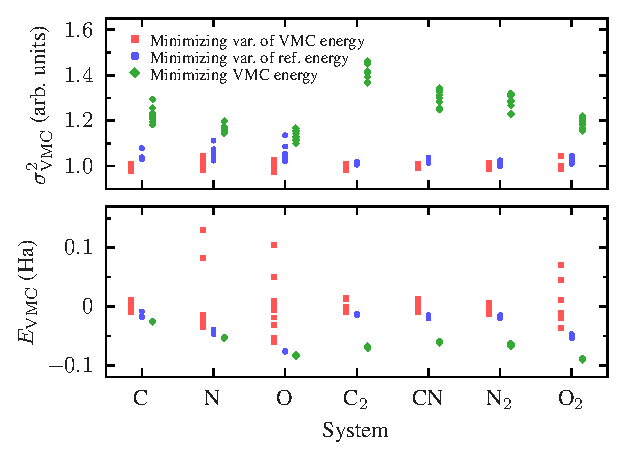
\includegraphics[width=0.8\textwidth]{figures/optimisation/Fig/varmin-E-Eref}
    \caption{Variance of the VMC energy (top) and VMC energy (bottom) of the systems considered in this chapter using the \vtz basis and Jastrow factors obtained by minimising the variance of the VMC energy (red squares), the variance of the reference energy (blue circles), or the VMC energy (green diamonds) in each of ten independent optimisation runs with $n_\mathrm{opt}=10^5$ VMC configurations. To ease comparisons, variances have been rescaled and energies shifted by their average values from minimising the variance of the VMC energy (i.e. the red squares average to a variance of $1$ and an energy of $0$ in the plot). The subpar ability of VMC energy variance minimisation to yield consistent VMC energies is evident in the bottom panel, suggesting to use the variance of the reference.}
    \label{fig:varmin-E-Eref}
\end{figure}
%
Minimizing the variance of the VMC energy produces lower average
values of $\sigma_\mathrm{VMC}^2$, as one would expect, but also erratic
VMC energies with very large standard deviations (up to $\sim50$ mHa
in our tests).
%
Minimizing the variance of the reference energy, on the other hand,
produces values of $\sigma_\mathrm{VMC}^2$ which are only slightly higher
on average than those obtained from minimizing the variance of the VMC
energy ($1$--$5\%$ in our tests), while producing more stable VMC
energies with much smaller standard deviations (up to $\sim3$ mHa in
our tests).
%
We therefore do not use ``regular'' variance minimization since it
introduces large stochastic noise, making it unsuitable for optimizing
Jastrow factors, and from this point on we use the term ``variance
minimization'' to refer to the minimization of the variance of the
reference energy.

\subsection{Choosing an Appropriate Sample Size}

\todo{...}

\subsection{Energy Minimisation}

\todo{...}


\section{Grid Sizes}
\todo{discuss the grid size (section III.C)}
\todo{...}


\section{Compactification of the CI Vector}
\todo{talk about compactness}

\section{Atomisation Energies}

\section{Neglecting Three-Body Excitations}

\todo{...}
\todo{mention Pauli exclusion principle as an argument for why this is a valid approximation (maybe use a figure?)}

\section{Conclusion and Outlook}
\todo{mention this is the way we now optimise Jastrow factors, but there is an important extension to the no-3-body approximation, xTC. Briefly describe.}
\todo{...}

\subsection{The xTC Approximation}

\todo{...}

\label{sec:xtc}

% optimization paper
% different objective functions for optimizing the Jastrow factor
% "hat" functions
% no-3-body approximation (performance benchmarking)
% xTC approximation

% ch 5
\chapter{The Transcorrelated Method for Multi-Reference Problems}
  \label{chap:binding}
\todo{...}

This chapter is based in large part on the following paper:\\
\fullcite{haupt_sizeconsistent}

Some images have been reused from this paper (with permission), clearly indicated in their figure labels.

% size consistency/binding curve paper
% jastrow factor forms (DTN, BH)
% present problem that arises when trying to apply previous method to binding curves
% present how the problem exists even with xtc
% the sign problem in TC
% trial wave functions
% hydrogen chains? xTC-DCSD

% ch 6
\chapter{The PyTCHInt Library}
\label{chap:pytchint}
\todo{...}

% the pytchint library
% library, integrals, how it works (see Aron's notes, paper)
% xtc implementation
% many options
% deterministic optimisation
% benchmarking?
% Python package

\chapter{Summary and Outlook}
  \label{chap:sumandout}

Transcorrelation has recently enjoyed somewhat of a revival since its early development in the 1960s, particularly when combined with other methods such as \gls{CC}, \gls{DMRG}, or \gls{FCIQMC}. The topic of this dissertation has been to further explore modern developments of the \gls{TC} method, especially applied to FCIQMC. Both of these methods combine ideas from \gls{QMC} and apply them to wave function methods. FCIQMC stochastically samples the (ground state) wave function of a system in analogy to \gls{DMC} to give \gls{FCI}-accuracy. The TC method adopts the Jastrow factor typically encountered in \gls{VMC} to correlate the electrons and explicitly take into account analytically-known behaviour at coalescence, a task difficult for conventional methods. Combining the two results in an essentially-exact stochastic method with rapid convergence towards the \gls{CBS} limit.

The primarily contributions to this field represented in this dissertation are threefold. First, in \autoref{chap:opt}, using flexible Jastrow factors with VMC to minimise the variance of the reference energy is proposed and shown to result in not only highly-accurate energies with chemically-accurate atomisation energies with only the \vtz basis set (compared to \vxz{5} for non-TC-FCI), but it also compactifies the wave function, making it better suited to sampling methods such as FCIQMC.

Second, in \autoref{chap:binding} we have shown that the TC method was not able to accurately describe problems of strongly multireference character, such as the dissociation of N$_2$, despite using FCIQMC after Jastrow-factor optimisation. Modifying the TC ansatz to accommodate multireference wave functions, we show that we can still benefit from using the TC method even in such challenging problems. Moreover, this introduces additional flexibility in the optimisation procedure, allowing us to tailor our Jastrow factor for specific states. We showed that this can be used to determine excited state energies with high accuracy.

Finally, in \autoref{chap:universal} we consider alternative forms for the Jastrow factor, either allowing much faster optimisation or bypassing it altogether, implying better suitability for larger systems. We considered two different categories of such Jastrow factors. In the first, the Jastrow factors were in a sense minimal, insofar as primarily handling known analytical behaviour of the wave function near coalescence points. These Jastrow factors were shown to sometimes result in nonvariational energies, but they did nevertheless exhibit favourable error cancellation. This is suggestive for future studies to prevent the nonvariational energies from occurring, possibly by optimising the cutoff range of the Jastrow factor terms. The second category of Jastrow factors were the atomic Jastrow factors, wherein the Jastrow factors are optimised for each atom in the system, and then these Jastrow factors are used in the molecule, only reoptimising a small portion of the parameters. This still resulted in clearly-superior basis-set convergence compared to conventional methods, while not requiring as much computational effort as the full optimisation. Moreover, the energies we found were all above the CBS limit. In principle, this opens the possibility of optimising sophisticated Jastrow factors for atoms across the periodic table, storing them in a database, and querying it when needed in a calculation, in analogy to what is already done with basis sets.

The methods proposed in this thesis have already been applied in other studies, such as applying TC to larger atoms\supercite{filip_2ndrow} or combining TC with \glspl{ECP} (where the FCIQMC-Jastrow approach of \autoref{chap:binding} can also be used).\supercite{simulaEcp} Other potential avenues of research include applying the methodologies to larger systems, such as solids, or embedding with the TC method. Combining the optimisation procedure outlined in \autoref{chap:opt} with the active space multireference approach in \autoref{chap:binding}, we could conceivably optimise biorthogonal orbitals in a transcorrelated CASSCF-like procedure for high accuracy within an active space. This might also be combined with simpified Jastrow factors such as those presented in \autoref{chap:universal} and deterministic optimisation as in \autoref{chap:pytchint} to allow for more robust but scalable calculations.

Despite having its roots in the 1960s, the methodology is still in its infancy, and as a result the most productive step forward would likely be to simply apply the methodology to new problems of chemical interest. This would necessarily lead to new methods, computational techniques, and code optimisations.

% solids, ecps, deterministic optimisation, tc-casscf, etc.
% focus on pytchint

\listoffigures
\listoftables
\printbibliography
\appendix
\chapter{Appendix (todo)}

\todo{Not sure what will be needed in appendices.}
% \section{sec}
% \subsection{subsec}
% \label{app:}

\chapter{Curriculum vitae}
  \label{Chap:CV}

  \section*{Education}
  \begin{small}
    \begin{tabular}{L{2.5cm}L{10cm}}
      \textbf{2020 -- 2025} & PhD student, Theoretical Chemistry\\
             & Max Planck Institute for Solid State Research, Stuttgart, Germany \\
             & \textbf{Thesis:} \thetitle \\
             & \textbf{Advisors:} Prof Ali Alavi \\
      \\
      \textbf{2014 -- 2019} & Bachelor of Science, Honours Physics and Mathematics, Minor in Computer Science\\
                  & University of British Columbia, Vancouver, Canada \\
             & \textbf{Thesis:}  Effects of Anisotropic Long-Range Hopping on Anderson Localization\\
             & \textbf{Advisor:} Prof Roman Krems \\
      \\
    \end{tabular}
  \end{small}

% \clearpage

\section*{Publications}
\begin{refsection}
\setmaxcitenames{10}

\begin{singlespace}
\begin{footnotesize}

\todo{Not really sure if there is a point to including a publications list...}

% \subsection*{First authored}
% \todo{publications, I guess: optimization paper, binding curve paper, pytchint paper (likely with a "to be submitted")}
% \begin{enumerate}[label=(\arabic*), itemindent=-0.5em]
%     \item \fullcite{hauptOptimizingJastrowFactors2023a}
%     \item \fullcite{haupt_sizeconsistent}
%     \item \fullcite{tchint}
% %   \item \fullcite*{..}
% \end{enumerate}

% \subsection*{Co-authored}
% \todo{publications, I guess: ECPs, 2nd row atoms, deterministic optimisation, spin-dependent Jastrows}
% \todo{Pablo's surname doesn't appear correctly in some of these}
% \begin{enumerate}[resume, label={(\arabic*)}, itemindent=-0.5em]
%     \item \fullcite{filip_2ndrow}
%     \item \fullcite{simulaEcp}
%     % \item \fullcite{filip_deterministic}
% %   \item \fullcite*{...}
% \end{enumerate}

\end{footnotesize}
\end{singlespace}

\end{refsection}
\end{document}
